\section{Experiments}
\label{sec:main-experiments}

This section provides empirical demonstration of the proposed theories. Appendix~\ref{sec:appendix-experiments} gives the simulation details. Fig.~\ref{fig:scenarios} illustrates the causal diagram of every scenario in which the true effect is known, and each analysis below reads its setting from that diagram. We estimate the average treatment effect $\tau$ through PROBE (Algo.~\ref{alg:probe-search}), and report the mean absolute error (MAE) over independently generated data sets.

We compare PROBE with various other methods. CEVAE \citep{louizos2017causal} learns a latent variable from all of $(X,W)$. Two further methods adjust for $(X,W)$ and for $X$ alone. For image proxies, the pixel CNN adjusts for a representation that a convolutional network \citep{lecun1998gradient} learns from all pixels. None of these methods holds out a block or checks balance. The remaining methods need the role of each proxy, which the diagram determines. Proximal two-stage least squares (2SLS) \citep{tchetgen2024ProximalCausalInference} needs a treatment-side proxy, which may point into $A$ but not into $Y$, and an outcome-side proxy, which may point into $Y$ but not into $A$ (Fig.~\ref{fig:causal-structures}(c)); single-proxy control \citep{park2024single} and its kernel version KSPC \citep{xu2025kernel} need one proxy of the untreated outcome $Y(0)$. We run each of these three methods once with the roles of the true diagram and once with wrong roles. An oracle that adjusts for $(X,U)$ blocks the path $A\leftarrow U\rightarrow Y$ directly and serves as a reference. In the chest X-ray diagrams (Fig.~\ref{fig:scenarios}(d), (e)), the proxy $W$ is one chest X-ray per unit and there are no covariates, so adjustment for $X$ is the difference in means; there PROBE is compared with adjustment for $X$, the pixel CNN, and the oracle.

\begin{figure}[t]
\centering
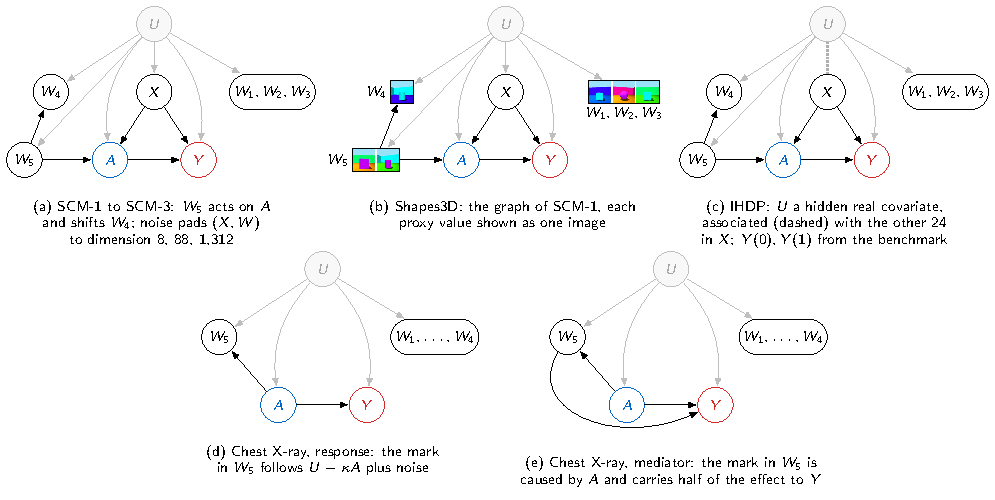
\includegraphics[width=\linewidth]{probe-scenario-dags.pdf}
\caption[Causal diagrams of the experiments.]{Causal diagrams of the experiments. The hidden confounder $U$ is gray, the treatment $A$ blue, and the outcome $Y$ red; the dashed line in (c) is an association between real covariates.}
\label{fig:scenarios}
\end{figure}

\paragraph{Synthetic Data Analysis.} In our example scenario (Fig.~\ref{fig:scenarios}(a)), a hidden severity $U$ affects both the treatment and the outcome, and the true effect is $\tau=1$. $U$ also affects the covariates $X$, which affect $A$ and $Y$. The proxy has five blocks, and $U$ points into each of them. Blocks $W_1$, $W_2$, and $W_3$ receive no other edge: they are noisy measurements of $U$ and are valid held-out blocks, each satisfying Assumptions~\ref{ass:joint-latent-exchangeability} and~\ref{ass:outcome-relevant-completeness}. Block $W_5$ also points into $A$, so it violates held-out treatment independence (Assumption~\ref{ass:joint-latent-exchangeability}), and no representation can balance it. Block $W_4$ points into neither $A$ nor $Y$ but is shifted by $W_5$; it can be balanced but violates outcome-relevant completeness (Assumption~\ref{ass:outcome-relevant-completeness}), so it points to a wrong effect. PROBE is not told which blocks are valid, whereas the role-requiring methods are given the correct roles in their correct-role runs. The proxy is a vector, high-dimensional in SCM-2 and SCM-3. The methods that need roles are told which coordinates form each block; PROBE is not, and finds the blocks from $W$ alone, before it sees $A$ or $Y$ (Appendix~\ref{sec:appendix-block-discovery}). We generate $100$ data sets of size $n=24{,}000$ for each setting.

\begin{figure}[t]
\centering
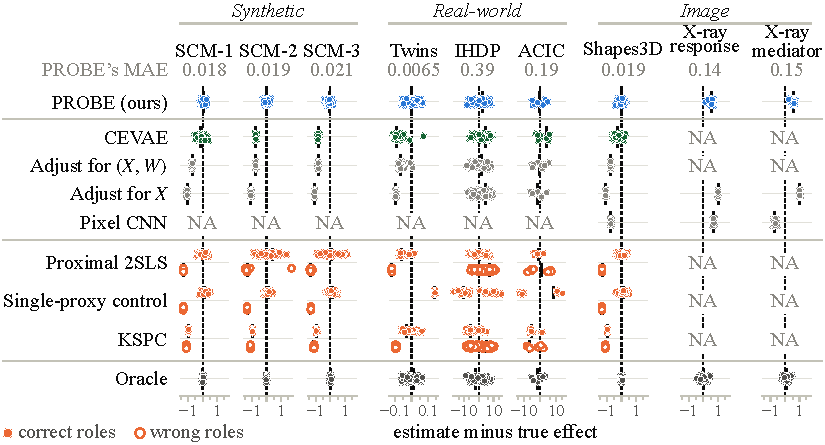
\includegraphics[width=\linewidth]{probe-experiments-v7.pdf}
\caption[Errors in the synthetic, real-world, and image data.]{Estimate minus the true effect on a symmetric log scale; each dot is one data set. Filled and hollow dots show methods that need proxy roles with correct and wrong roles; on the real-world data, single-proxy control is used as an ATE estimator. In the synthetic and real-world panels PROBE finds the blocks from $W$ (Appendix~\ref{sec:appendix-block-discovery}); in the image panels the blocks are given.}
\label{fig:experiments}\label{fig:synthetic}\label{fig:realdata}
\end{figure}
Fig.~\ref{fig:synthetic} (Synthetic) shows that PROBE, without being told the roles or the blocks, stays near zero error in all three settings, while CEVAE degrades as the dimension grows and adjustment for $(X,W)$ or $X$ stays biased.

\paragraph{Real-World Data Analysis.}\label{sec:real-world-analysis} We use four real-world data sets. Twins \citep{louizos2017causal}, IHDP \citep{hill2011bayesian}, and ACIC 2016 \citep{dorie2019automated} are semi-synthetic benchmarks built on real covariates, with $11{,}984$, $747$, and $4{,}802$ units and $42$, $24$, and $78$ covariates. In each, we hide one covariate as $U$ and generate the proxies and the treatment from it with one fixed recipe, so the effect is known exactly. Fig.~\ref{fig:scenarios}(c) shows the resulting graph: the proxies and the treatment follow the graph of the synthetic scenario, the hidden covariate $U$ is associated with the remaining covariates $X$ instead of being their cause, and the potential outcomes are those of the benchmark. We also analyze the right heart catheterization (RHC) study \citep{connors1996effectiveness}, an observational study with no ground truth; because Fig.~\ref{fig:experiments} compares methods only where the true effect is known, the RHC analysis is in Appendix~\ref{sec:appendix-rhc}.

Fig.~\ref{fig:realdata} (Real-world) shows that PROBE, without being told the roles or the blocks, is the most accurate method on Twins and among the three most accurate on IHDP and ACIC. Methods that need the roles are accurate only with the correct roles and degrade sharply with wrong ones.

% wrapfig cannot follow a run-in \paragraph heading (both use \everypar), so this heading is set by hand in the
% \paragraph style of KOMA-Script: the same space above, font, and run-in gap.
\par\addvspace{3.25ex plus 1ex minus .2ex}
\begin{wrapfigure}{r}{2.78in}
\centering
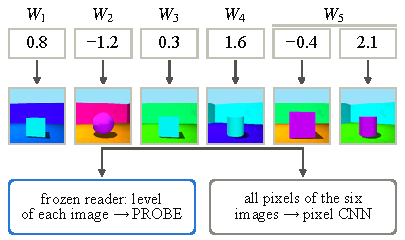
\includegraphics[width=2.70in]{probe-shapes3d-diagram.pdf}
\captionsetup{format=plain}
\caption[Shapes3D setting.]{Shapes3D setting: each proxy value of a unit sets the orientation of one Shapes3D image.}
\label{fig:shapes3d}
\end{wrapfigure}
\noindent{\usekomafont{disposition}\usekomafont{paragraph}Shapes3D Analysis.}\hspace{1em}In this scenario (Fig.~\ref{fig:scenarios}(b)), the true effect is $\tau=1$, $W_1$, $W_2$, and $W_3$ are valid held-out blocks, and $W_4$ and $W_5$ are not. Here every proxy block is made of images. Each unit is first generated as in SCM-1. The hidden confounder $U$ itself is never observed; what is generated from it are six proxy values, one in each of $W_1$ to $W_4$ and two in $W_5$. The values in $W_1$ to $W_3$ are noisy measurements of $U$. The two values in $W_5$ mix a measurement of $U$ with a second value that affects only the treatment, and the value in $W_4$ is a measurement of $U$ shifted by that second value, which is why $W_4$ and $W_5$ are not valid held-out blocks. Each proxy value is then shown as an image instead of a number. Shapes3D \citep{3dshapes18} is a collection of $64\times64$ images of an object in a room whose colors, shape, size, and orientation vary; for each proxy value we take one such image whose orientation, the angle at which the scene is turned, equals the value rounded to one of $15$ angles, and whose colors, shape, and size are random. A unit's proxy is therefore six images, one in each of $W_1$ to $W_4$ and two in $W_5$, and the analyst sees only their pixels (Fig.~\ref{fig:shapes3d}; SCM-4 in Appendix~\ref{sec:appendix-image-rendering}). To use these images, PROBE first turns each one back into its proxy value with an image reader, a convolutional network trained beforehand on other Shapes3D images to recognize the orientation, which reads every image of this experiment correctly. It then runs on the six recovered values as in SCM-1. The pixel CNN instead adjusts for a summary that it learns from all pixels of the six images, including the images of $W_4$ and $W_5$. We generate $100$ data sets of size $n=24{,}000$. Fig.~\ref{fig:experiments} (Image, Shapes3D) shows that PROBE, without being told the roles, has an MAE of $0.019$, as in SCM-1, while adjustment for $(X,W)$ has an MAE of $0.31$ and the pixel CNN, which reads every pixel but never checks balance, $0.29$.

\paragraph{Chest X-ray Analysis.}\label{sec:single-image} In this scenario, a hidden severity $U$ affects both the treatment and the outcome, the true effect is $\tau=1$, the proxy $W$ is one of $5{,}856$ pediatric chest X-rays \citep{kermany2018identifying,yang2023medmnist}, and $U$ is the score of a pneumonia classifier on that X-ray. The image is cut into five blocks, and $U$ points into each of them (Fig.~\ref{fig:scenarios}(d), (e)). The lung quadrants $W_1$ to $W_4$ receive no other edge and satisfy held-out treatment independence (Assumption~\ref{ass:joint-latent-exchangeability}), and the central strip $W_5$ violates it, because $A$ also points into it: the mark in $W_5$ is either a response that follows $U-\kappa A$ plus noise, so that $A$ and $U$ both point into $W_5$ (d), or a mediator that passes half of the effect on to $Y$, so that $A$ points into $W_5$ and $W_5$ into $Y$ (e). PROBE is not told which block carries the mark and screens one block at a time (Appendix~\ref{sec:appendix-single-image}); the pixel CNN adjusts for all five blocks. We generate $50$ data sets for each scenario.

\begin{figure}[tb]
\centering
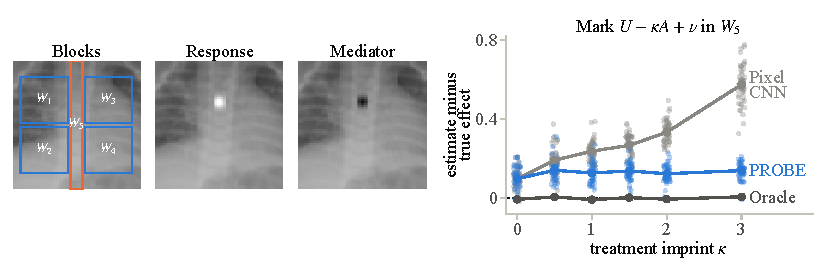
\includegraphics[width=\linewidth]{probe-single-image-v3.pdf}
\caption[Chest X-ray proxy.]{Left: the five blocks of one chest X-ray, and the same X-ray with a response mark and with a mediator mark in $W_5$. Right: estimate minus the true effect as the treatment's imprint $\kappa$ grows; $50$ data sets per value.}
\label{fig:single-image}
\end{figure}

Fig.~\ref{fig:experiments} (Image, X-ray) shows that PROBE hides $W_5$ in all $50$ data sets, with an MAE of $0.14$ under the response and $0.15$ under the mediator, against $0.27$ and $0.26$ for the pixel CNN. As the imprint $\kappa$ grows from $0$ to $3$ (Fig.~\ref{fig:single-image}, right), the MAE of the pixel CNN grows from $0.10$ to $0.57$, as Prop.~\ref{prop:single-image-decomposition}(b) predicts, while that of PROBE stays between $0.10$ and $0.14$; Appendix~\ref{sec:appendix-single-image} reports the other scenarios.
